\section{Method}
\label{sec:method}

\sys constructs reusable, code-anchored optimization memory from expert evidence. Guided deoptimization walks an expert kernel backward but stores accepted steps as inverse forward transitions (\autoref{sec:method-deopt}); a lift turns recurring transitions into candidate skill hypotheses (\autoref{sec:method-extract}); held-out roundtrip materialization decides which hypotheses become reusable skills (\autoref{sec:method-use}). 

\subsection{Motivation}
\label{sec:method-formulation}

\begin{figure*}[t]
\centering
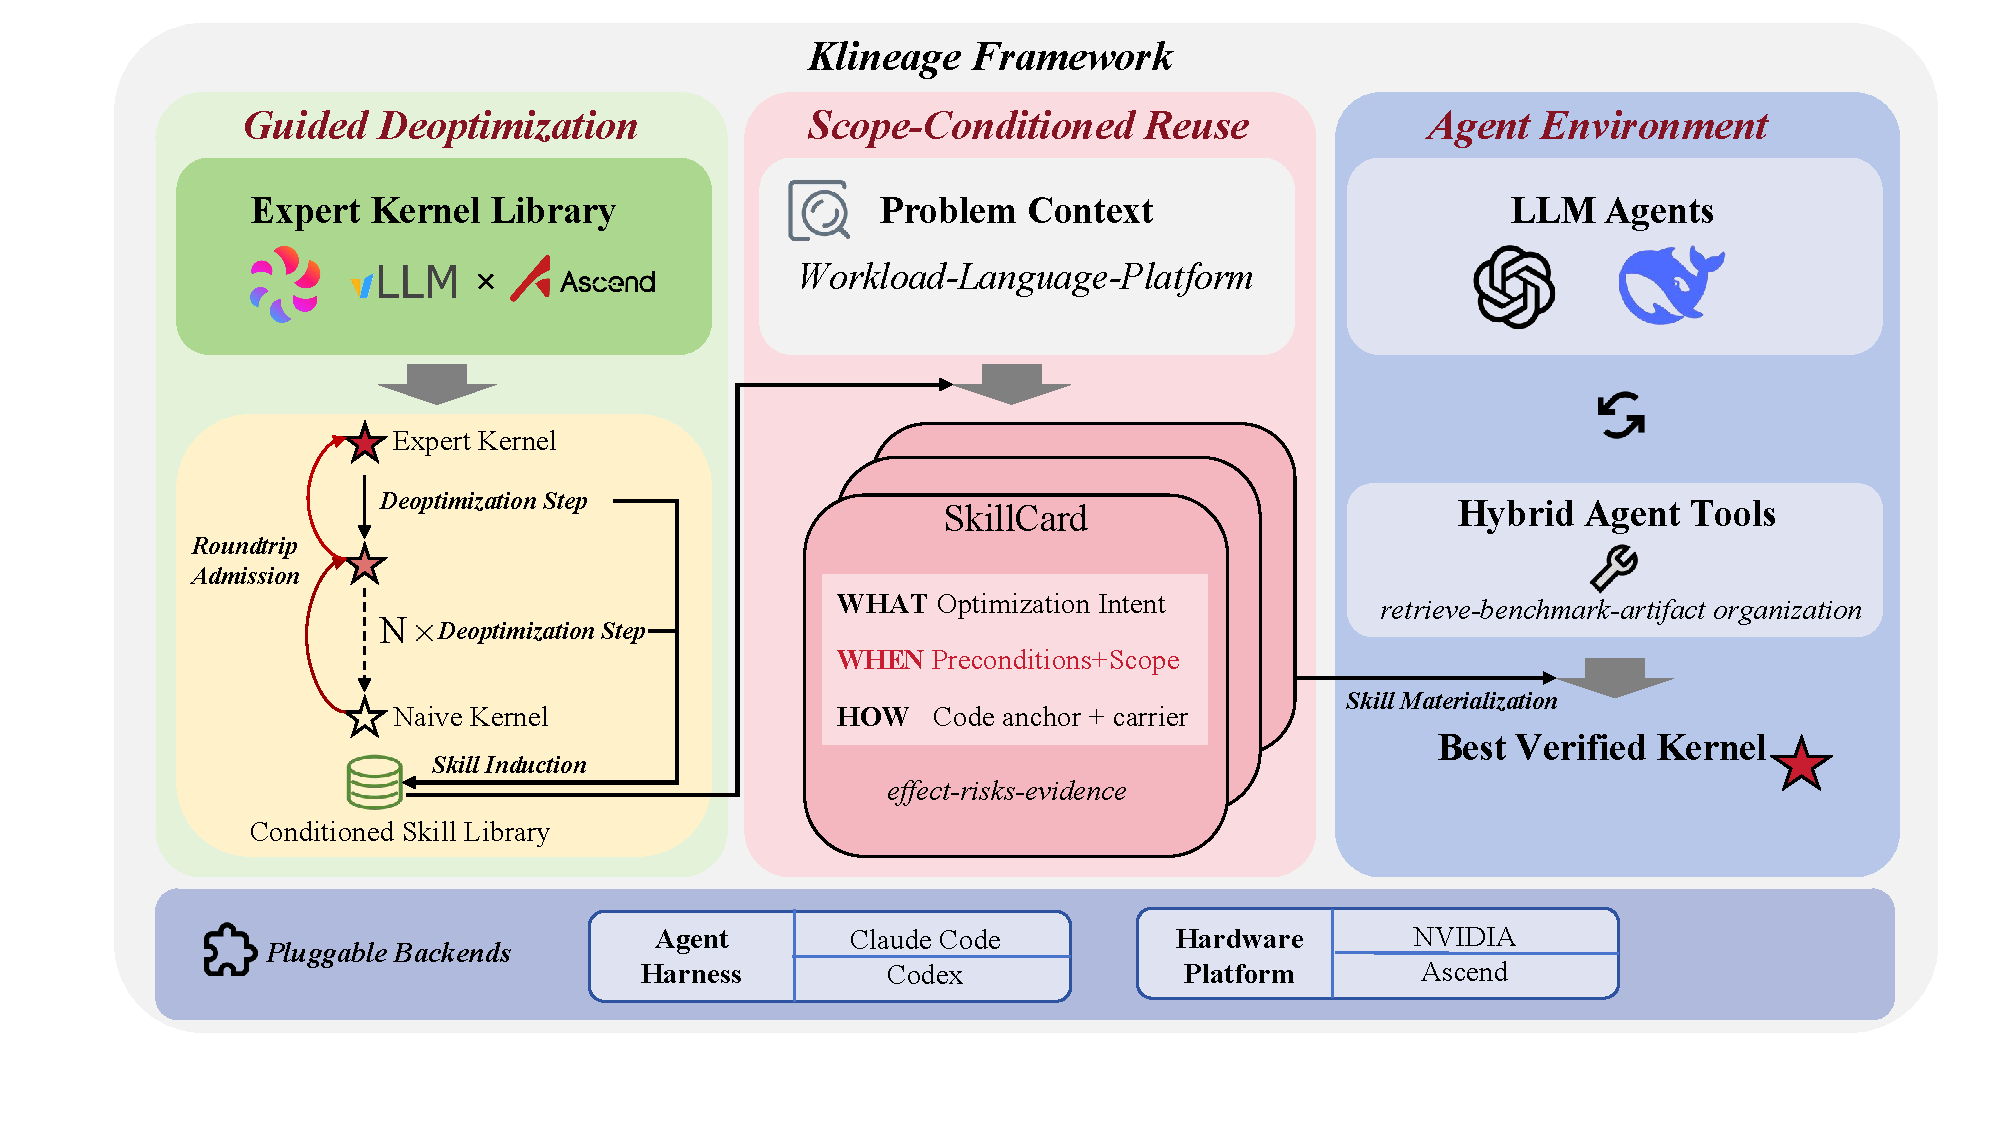
\includegraphics[width=\textwidth]{overview.pdf}
\caption{\small Overview of \sys{}.}
\label{fig:method-overview}
\end{figure*}

As illustrated in \autoref{fig:lineage-teaser}, expert kernels entangle many compatible optimization decisions, and walking them backward under validation exposes each decision as an explicit forward transition. This direction is more natural in practice because high-quality expert kernels in existing repositories are often not paired with corresponding naive implementations. We make this construction precise below.
% Original wording (kept for ease of restoration): LLM kernel agents often know \emph{what} optimizations to try, but not reliably \emph{when} they are valid. Vectorized loads require alignment and tail handling; pipelines require staged data movement; hardware intrinsics require matching tiles, layouts, and platforms. Forward rollouts expose such preconditions only along the states an agent reaches. Expert kernels provide denser evidence: their final code entangles many compatible decisions whose validity can be exposed by walking the kernel backward through validated simplifications.

\sys represents this evidence at three levels as shown in ~\autoref{fig:lineage-teaser}(b). A \emph{backward deoptimization step} $b_i : K_i \rightarrow K_{i-1}$ removes or weakens one optimization and records the edit, locus, and validation evidence for the simplified predecessor. \sys stores the inverse $\tau_i = b_i^{-1}:K_{i-1}\rightarrow K_i$ as a \emph{forward concrete transition}: a validated before/after edit from a simpler state toward the expert state. A \emph{lineage} is the resulting forward sequence
\[
L = (K_0, \tau_1, K_1, \ldots, \tau_n, K_n = K^*),
\]
an executable curriculum from naive to expert, not a claim about the expert's historical writing path.

Concrete transitions are still tied to one source kernel. \sys lifts them into an \emph{optimization intent}: the abstract pass family being expressed, such as staging reused tiles, vectorizing aligned contiguous loads, or exposing tunable parameters. A \emph{candidate skill hypothesis} $\hat{\sigma}$ makes the intent actionable by adding a code/IR anchor, a carrier, conditions, and evidence:
\[
\begin{aligned}
\hat{\sigma} = \big(&\iota,\, \mathrm{anchor},\, \mathrm{carrier},\, \mathrm{pre},\\
                   &\mathrm{effect},\, \mathrm{evidence},\, \mathrm{risk},\,
                    \mathrm{scope},\, \mathrm{ver}\big),
\end{aligned}
\]
where $\iota$ is the intent, $\mathrm{anchor}$ identifies the code or IR surface on which it acts, and $\mathrm{carrier}$ is an actionable but not necessarily executable representation such as a diff sketch, pseudocode, annotated kernel snippet, schedule fragment, or natural-language code annotation. The other fields record preconditions, expected effects, evidence, risks, scope over case/language/platform/prior-action context, and a verification log $\mathrm{ver}$ (\autoref{sec:method-extract}). A hypothesis becomes an admitted \emph{skill} only after at least one trial succeeds.
% Original wording (kept for ease of restoration): The verification log is a set of held-out roundtrip trials (\autoref{sec:method-extract}) in which an agent re-materialized the candidate skill on a fresh state; each trial records the trial case, the resulting submission, and whether the compile/correctness/profile gate accepted the materialization.
At reuse time, an agent \emph{materializes} the skill on a target code surface; the candidate is accepted only if it passes the compile/correctness/profile gate.

\subsection{Guided Deoptimization}
\label{sec:method-deopt}

Starting from $K_n = K^*$, \sys repeatedly proposes a simplification (e.g., remove software pipelining, devectorize, scalarize an intrinsic), patches the kernel with an LLM rewriter, and accepts the patch only if it passes validation. The inverse of an accepted simplification becomes a forward transition in the lineage; rejected simplifications become precondition-violation evidence for later $\mathrm{risk}$ fields.

\paragraph{Operationalizing $\tau_i = b_i^{-1}$.}
The forward transition $\tau_i$ is not a textual reversal of the diff that produced $b_i$. The LLM rewriter re-derives a forward edit on $K_{i-1}$ functionally equivalent to $K_i$, given the action category and locus from the backward step. The candidate forward edit is then run through the compile/correctness/profile gate; only edits whose output kernel matches $K_i$'s validation status are stored as $\tau_i$. This makes $\tau_i$ an executable forward primitive grounded in $K_{i-1}$'s state, not a syntactic inversion that may not even compile.
% Original wording (kept for ease of restoration): After a backward step from $K_i$ to $K_{i-1}$ is accepted, the LLM rewriter is asked to re-derive a forward edit that takes $K_{i-1}$ to a kernel functionally equivalent to $K_i$ on the same shape and dtype, given the action category, the locus identified by the backward step, and the surface code of $K_{i-1}$.

During induction we group accepted backward steps by action category to anchor the lift, over an open vocabulary rather than a closed set of actions. Multiple intents may be lifted from one category, the same intent may admit different carriers in different languages, and any partial order over actions is treated as a soft prior: if a simplification violates the order but still passes validation, its inverse transition is kept.

\subsection{From Transitions to Skills}
\label{sec:method-extract}

The library is induced from forward concrete transitions. Transitions sharing an action category and similar locus / effect signatures are aggregated, and an LLM receives their forward diffs, loci, profile deltas, and local code context, then lifts them into an intent $\iota$, an anchor, a carrier, and a portable $(\mathrm{pre}, \mathrm{effect}, \mathrm{risk})$ tuple. The intent describes the manipulated code construct and exploited platform property; the anchor and carrier keep it actionable.

\paragraph{Intent, carrier, and materialization.}
The lift separates the general idea from its realization. The intent names the optimization, the carrier gives it a code-bearing form, and materialization instantiates the admitted skill on a target language and code surface. One intent can therefore have different realizations across cases, languages, and platforms.

\paragraph{Roundtrip admission.}
An induced $\hat{\sigma}$ starts as a hypothesis. Admission requires at least one held-out roundtrip in which an agent, given only $\hat{\sigma}$, materializes it on a fresh state and reproduces its expected effect; success is recorded in $\mathrm{ver}$. Only admitted skills $\sigma \in \mathcal{S}$ are reused.

% ============================================================================
% REMOVED 2026-09-25 at the author's request: the skill-intent table.  Ten
% two-word conditions understated the very thing the paper is about, and the
% schema is already defined in this section.  If space allows, one rendered
% SkillCard with its real preconditions would serve better than this table.
% ============================================================================
% \begin{table}[t]
% \centering
% \small
% \setlength{\tabcolsep}{3pt}
% \begin{tabular}{@{}lll@{}}
% \toprule
% \textbf{Skill intent} & \textbf{Constraint} & \textbf{Prior action} \\
% \midrule
% \texttt{tile / sm\_stage}     & any       & loops over output       \\
% \texttt{vectorize\_global}    & any       & 128-bit aligned access  \\
% \texttt{cp.async + pipeline}  & NV-A+     & sm-staged               \\
% \texttt{tma\_load}            & NV-H+     & descriptor encoded      \\
% \texttt{warp\_specialize}     & NV-H+     & producer/consumer split \\
% \texttt{mma (m16n8k16)}       & NV-A+     & tile fits mma           \\
% \texttt{smem\_transpose}      & any       & strided scan axis       \\
% \texttt{gemm\_phase\_decomp.} & any       & per-token GEMM          \\
% \texttt{templatize}           & any       & const at tunable slot   \\
% \texttt{autotune}             & T/TL/CU$^\dagger$ & templatized       \\
% \bottomrule
% \end{tabular}
% \caption{Skill intents induced from our five expert kernels. ``Constraint'' is the language and
% platform the intent is verified on; ``prior action'' is the state the kernel must already be in for
% it to apply. $\dagger$: native autotuning in Triton and TileLang, explicit autotuning in CUDA.}
% \label{tab:actions}
% \end{table}


\subsection{Scope-Conditioned Reuse}
\label{sec:method-use}

\sys supplies a verified, scope-conditioned candidate pool rather than a new search policy. Given a target $T$ and a root submission, the downstream agent selects admitted skills, materializes them on the target code surface, and submits candidates under the same fixed-budget compile/correctness/profile loop used by all baselines. In the online prompt, each retrieved SkillCard is serialized as the fields in $\hat{\sigma}$---intent, anchor, carrier, precondition, effect, evidence, risk, scope, and verification log---with the carrier copied verbatim as the code-bearing hint to instantiate, not as an executable tool. The root submission may be a compiler baseline, a partially optimized agent attempt, or a previous best kernel.
% Original wording (kept for ease of restoration): The root submission may be a compiler baseline, a partially optimized agent attempt, or a previous best kernel; retrieved skills then serve as an expert intent reference, and the agent identifies which intents are already present, missing, or mis-materialized.
To bound the candidate pool, \sys retrieves with a multi-faceted retriever: given $T = (c_T, l_T, p_T, d_T)$, it returns the union of per-dimension top-$k$ skills under similarities over $(\mathcal{C}, \mathcal{L}, \mathcal{P}, \mathcal{D})$, using each skill's verified rather than declared scope.

\subsection{\sys Framework}

Building on these ideas, we implement \sys as an agent framework for GPU kernel programming. As shown in \autoref{fig:method-overview}, \sys induces conditioned skills from expert-written kernels such as FlashInfer~\cite{ye2025flashinfer} through guided deoptimization. Each skill records not only an optimization, but also the conditions under which it applies, such as data layout, hardware features, memory placement, and pipeline schedule. Given a new workload with the specified language and target platform, \sys guides LLM agents to retrieve and materialize skills whose conditions match the current context. We also provide hybrid agent tools for LLM Agents in the environment, including shared interfaces for skill retrieval, kernel artifact organization, and benchmarking, together with platform-specific profiling tools such as \texttt{ncu} and \texttt{msprof}. \sys{} also provides a unified abstraction for pluggable integration of different backends and agent harnesses. This design makes agent trajectories and generated artifacts traceable while leaving agents free to profile kernels, diagnose bottlenecks, and explore platform-specific optimizations.
